%%% Ne pas modifier jusqu'à la ligne 25
\documentclass[a4paper,12pt]{book}
\usepackage[utf8]{inputenc}
\usepackage[french]{babel}
%%\usepackage{CJK}
\usepackage{yhmath}
\usepackage[left=2cm,right=2cm,top=3cm,bottom=2cm, headheight=1.5cm,headsep=1.5cm]{geometry}
%%\usepackage{CJKutf8}
\usepackage{amsfonts}
\usepackage{mathrsfs}
\usepackage{amsmath,amsfonts,amssymb,dsfont}
\usepackage{graphicx}
\usepackage{subfigure}
\usepackage{enumitem}		%\enumerate-resume
\usepackage[colorlinks=true,unicode={true},hyperindex=false, linkcolor=blue, urlcolor=blue]{hyperref}
\newcommand{\myref}[1]{\ref{#1} page \pageref{#1}}

\addto\captionsfrench{\def\tablename{Tableau}}  %légendes des tableaux
\renewcommand\thesection{\Roman{section}~-~} 
\renewcommand\thesubsection{\Roman{section}.\Alph{subsection}~-~} 
\renewcommand\thesubsubsection{\Roman{section}.\Alph{subsection}.\arabic{subsubsection}~-~} 

\newcommand{\conclusion}[1]{\newline \centerline{\fbox{#1}}}

\setcounter{secnumdepth}{3}
\parindent=0pt

\usepackage{fancyhdr}
\pagestyle{fancy}

\lhead{SJTU-ParisTech} 
%%%%%%%%%%%%%%%%%%%%%%%%%%%%%%%%%%
\chead{DM5}
\rhead{Daniel 518261910024}

\begin{document}
\renewcommand{\labelitemi}{$\blacktriangleright$}
\renewcommand{\labelitemii}{$\bullet$}



\section{Exercice 1}
\subsection{}
Comme $X$ est une variable aléatoire discrète à valeurs dans $\mathbb{N}$, on a 
$$\forall k \in \{0,1,\cdots,n-1\}, (X>k)=(X>n) \cup \left(\bigcup_{i=k+1}^n (X=i)\right)$$
une union dénombrable disjointe, on a donc 
$$
\forall k \in \{0,1,\cdots,n-1\}, \mathbb{P}(X>k)=\mathbb{P}(X>n)+\sum_{i=k+1}^n \mathbb{P}(X=i)
$$
donc 
$$
\sum_{k=0}^{n-1}\left(\mathbb{P}(X>k)-\mathbb{P}(X>n)\right)=\sum_{k=0}^{n-1}\sum_{i=k+1}^n \mathbb{P}(X=i)
$$
à droite de l'équation, le terme $\mathbb{P}(X=k)$ est sommé pour $k$ fois, on a donc 
$$
\sum_{k=0}^{n-1}\sum_{i=k+1}^n \mathbb{P}(X=i)=\sum_{k=0}^n k\mathbb{P}(X=k)
$$
d'où 
$$
\boxed{\sum_{k=0}^n k\mathbb{P}(X=k)=\sum_{k=0}^{n-1}\mathbb{P}(X>k)-n\mathbb{P}(X>n)}
$$

\subsection{}
$$\forall n \in \mathbb{N}^{*}, \sum_{k=0}^n k\mathbb{P}(X=k)=\sum_{k=0}^{n}\mathbb{P}(X>k)-(n+1)\mathbb{P}(X>n) \leq \sum_{k=0}^{n}\mathbb{P}(X>k)$$
on sait que $\sum_k \mathbb{P}(X>k)$ converge, et car ils sont de termes positifs, on a $\sum_k k\mathbb{P}(X=k)$ converge aussi. 

On a donc la famille $\left(k\mathbb{P}(X=k)\right)_{k \in \mathbb{N}}$ est sommable, alors \fbox{$X$ admet une espérance}

\subsection{}
On pose $\forall n \in \mathbb{N}^{*}, u_n=n\mathbb{P}(X=n) \geq 0$. Car $X$ admet une espérance, alors la famille $(u_n)_{n \in \mathbb{N}^{*}}$ est sommable. 
C'est à dire la série à termes positifs $\sum u_n$ converge. 

On a donc $\boxed{n\mathbb{P}(X=n)=u_n\xrightarrow[n \to +\infty]{} 0}$. (sinon, la série diverge grossièrement)

Puisque on a $(X>n)=\bigcup_{i=n+1}^{+\infty}(X=i)$, car les probabilités sont positives, on a  
\begin{align*}
    \forall n \in \mathbb{N}^{*}, \sum_{k=0}^n k\mathbb{P}(X=k)&=\sum_{k=0}^{n-1}\mathbb{P}(X>k)-n\mathbb{P}(X>n)\\
                                 &=\sum_{k=0}^{n}\mathbb{P}(X>k)-(n+1)\mathbb{P}(X>n)\\
                                 &=\sum_{k=0}^{n}\mathbb{P}(X>k)-(n+1)\sum_{i=n+1}^{+\infty}\mathbb{P}(X=i)\\
                                 &\geq \sum_{k=0}^{n}\mathbb{P}(X>k)-\sum_{i=n+1}^{+\infty}i\mathbb{P}(X=i)
\end{align*}
d'où 
$$
\forall n \in \mathbb{N}^{*}, \sum_{k=0}^{+\infty} k\mathbb{P}(X=k) \geq \sum_{k=0}^{n}\mathbb{P}(X>k)
$$
Car $X$ admet une espérance, $\sum_{k=0}^{+\infty} k\mathbb{P}(X=k)$ converge, donc \fbox{$\sum_k \mathbb{P}(X>k)$ converge aussi}
(elle est une série à termes positifs est majorée)

Et on a 
$$
\mathbb{E}(X)=\sum_{k=0}^{+\infty} k\mathbb{P}(X=k)\geq \sum_{k=0}^{+\infty} \mathbb{P}(X>k)
$$
De plus, on a 
$$
\sum_{k=0}^n k\mathbb{P}(X=k)=\sum_{k=0}^{n}\mathbb{P}(X>k)-(n+1)\mathbb{P}(X>n) \leq \sum_{k=0}^{n}\mathbb{P}(X>k)
$$
quand $n$ tends vers l'infini, et car $\sum_k \mathbb{P}(X=k)$ converge, on a 
$$
\mathbb{E}(X)=\sum_{k=0}^{+\infty} k\mathbb{P}(X=k)\leq \sum_{k=0}^{+\infty} \mathbb{P}(X>k)
$$

Finalement, on a $\boxed{\mathbb{E}(X)=\sum_{k=0}^{+\infty} \mathbb{P}(X>k)}$

\section{Exercice 2}
On a $X \sim \mathscr{U}(0,n), Y \sim \mathscr{U}(0,n)$
\subsection{}
Pour $n \in \mathbb{N}^{*}$, on a $0 \leq Z \leq n$, donc $\mathbb{E}(Z)\leq \mathbb{E}(n)=n$, qui est finie. 
Donc \fbox{$Z$ admet une espérance}. 

Par la même méthode, $0 \leq Y \leq n$, \fbox{$Y$ admet une espérance}
\subsection{}
$\forall n \in \mathbb{N}^{*}$, on a 
$$
\mathbb{E}(|X-Y|)=\sum_{(i,j)\in \{1,\cdots,n\}^2}|i-j|\mathbb{P}(X=i,Y=j)
$$
car $X$ et $Y$ sont indépendantes, on a donc 
$$
\forall (i,j)\in \{1,\cdots,n\}^2, \mathbb{P}(X=i,Y=j)=\mathbb{P}(X=i)\mathbb{P}(Y=j)=\frac{1}{(n+1)^2}
$$
donc 
$$
\mathbb{E}(|X-Y|)=\frac{1}{(n+1)^2}\sum_{(i,j)\in \{1,\cdots,n\}^2}|i-j|
$$
par symétrie, on a 
$$
\sum_{(i,j)\in \{1,\cdots,n\}^2}|i-j|=2\sum_{i=0}^n\sum_{j=0}^i(i-j)
$$
donc 
\begin{align*}
    \mathbb{E}(|X-Y|)&=\frac{2}{(n+1)^2}\sum_{i=0}^n\sum_{j=0}^i(i-j)\\
    &=\frac{2}{(n+1)^2}\sum_{i=0}^n\sum_{k=0}^ik\\
    &=\frac{2}{(n+1)^2}\sum_{i=0}^n\frac{i(i+1)}{2}
\end{align*}
Finalement, on a $\boxed{\mathbb{E}(Z)=\frac{n^2+2n}{3n+3} \mathop{\sim}\limits_{n \to +\infty}\frac{n}{3}}$


\subsection{}
Par la même méthode, on a 
$$
\mathbb{E}(\min(X,Y))=\frac{1}{(n+1)^2}\sum_{(i,j)\in \{1,\cdots,n\}^2}\min (i,j)=\frac{1}{(n+1)^2}\sum_{i=0}^n\sum_{j=0}^n\min (i,j)
$$
On va montrer que $\forall n \in \mathbb{N}^{*}, \sum_{i=0}^n\sum_{j=0}^n\min (i,j)=\sum_{k=0}^n k^2$ par récurrence. 
\begin{itemize}
    \item $n=1$: $$\sum_{i=0}^1\sum_{j=0}^1\min (i,j)=\min(0,0)+\min(0,0)+\min(0,0)+\min(1,1)=1=\sum_{k=0}^1 k^2$$
    l'énoncé est vrai
    \item Supposons que l'énoncé est vrai pour rang $n$, c'est-à-dire 
    $$
    \sum_{i=0}^n\sum_{j=0}^n\min (i,j)=\sum_{k=0}^n k^2
    $$
    alors pour le rang $n+1$, 
    \begin{align*}
    \sum_{i=0}^{n+1}\sum_{j=0}^{n+1}\min (i,j)&=\sum_{i=0}^n\sum_{j=0}^n\min (i,j)+\sum_{i=0}^{n+1}\min(i,n+1)+\sum_{j=0}^{n+1}\min(n+1,j)-\min(n+1,n+1)\\
    &=\sum_{i=0}^n\sum_{j=0}^n\min (i,j)+2*\frac{(n+1)(n+2)}{2}-(n+1)\\
    &=\sum_{k=0}^n k^2+(n+1)^2\\
    &=\sum_{k=0}^{n+1} k^2
    \end{align*}
l'énoncé est aussi vrai
\end{itemize}
\begin{figure}[h]
    \begin{center}
    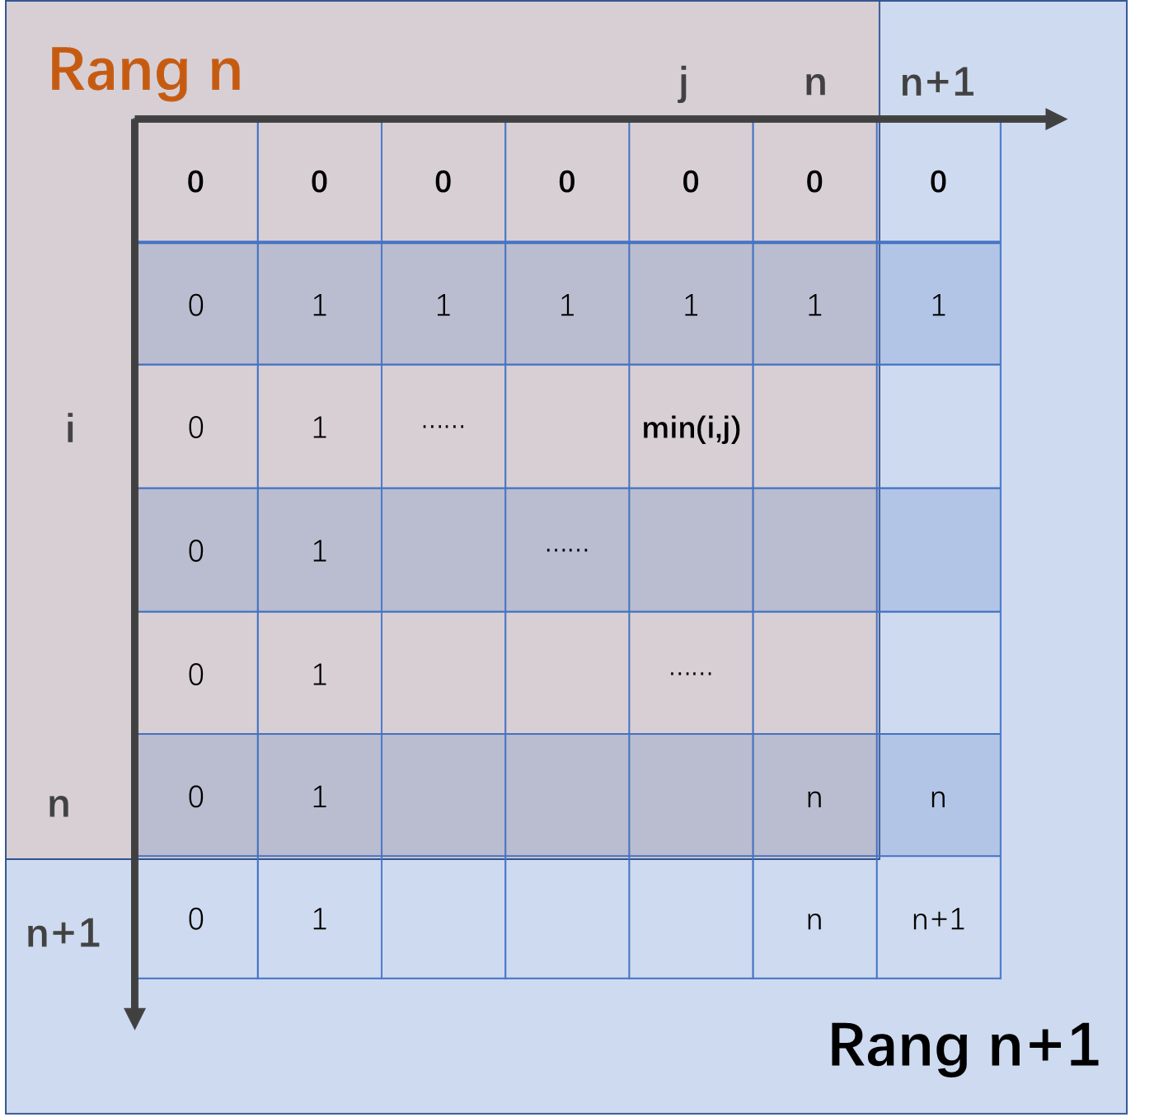
\includegraphics[scale=0.4]{mathdm52.png}
    \end{center}
    \caption{Sommation de l'équation}
\end{figure}
On a donc 
$$
\mathbb{E}(\min(X,Y))=\frac{1}{(n+1)^2}\sum_{k=0}^{n} k^2
$$
Finalement, $\boxed{\mathbb{E}(T)=\frac{2n^2+n}{6n+6}\mathop{\sim}\limits_{n \to +\infty}\frac{n}{3}}$


\section{Exercice 3}
\subsection{}
$f$ est continue par morceaux sur $\mathbb{R}$. $f$ est aussi intégrable: elle est nulle dehors $[1,+\infty[$, est intégral sur $[1,+\infty[$(intégral de Riemann). 
Pour que $f$ soit une densité, il faut que $\forall t \in \mathbb{R}, f(t) \geq 0$. 
Donc $a \geq 0$. 

De plus, il faut que $\int_{t \in \mathbb{R}} f(t)\,dt=1$, donc 
$$
1=\int_{t \in \mathbb{R}} f(t)\,dt=\int_1^{+\infty} \frac{a}{t\sqrt{t}}\,dt=a\left[-2t^{-\frac{1}{2}}\right]^{+\infty}_1=2a
$$
donc $\boxed{a=\frac{1}{2}}$
on a donc $\forall t \in \mathbb{R}, f(t)=\frac{1}{2t\sqrt{t}}1_{[1,+\infty[}(t)$
\subsection{}
On a 
$$
\forall I \subset \mathbb{R}, \mathbb{P}(X \in I)=\int_I f(t)\,dt
$$
donc 
$$
\forall x \in \mathbb{R}, F_X(x)=\mathbb{P} (X\leq x)=\int_{-\infty}^{x} f(t)\,dt
$$
\begin{itemize}
    \item si $x \leq 1$, on a $f(t)=0$, donc $F_X(x)=0$
    \item si $x > 1$, 
    \begin{align*}
        F_X(x)&=\int_{-\infty}^{x} f(t)\,dt=\int_{1}^{x} f(t)\,dt\\
              &=\int_{1}^{x} \frac{1}{2t\sqrt{t}}\,dt\\
              &=\left[-t^{-\frac{1}{2}}\right]^x_1\\
              &=1-x^{-\frac{1}{2}}
    \end{align*}    
\end{itemize}
on a donc 
\begin{equation}  \nonumber
    F_X(x)=\left\{  
                 \begin{array}{rcl}  
                 0 & & x \leq 1\\  
                 1-x^{-\frac{1}{2}} & & x > 1
                 \end{array}  
    \right.  
\end{equation} 
$F_X(x)$ est à valeurs dans $[0,1]$, $F_X$ est donc bien une fonction de répartition. 
\begin{figure}[h]
    \begin{center}
    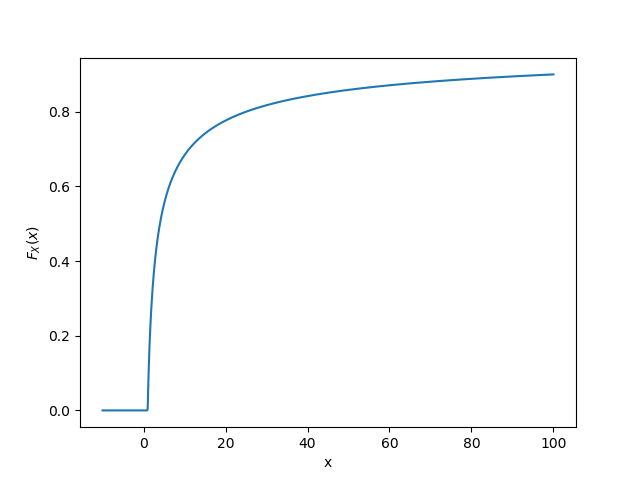
\includegraphics[scale=0.5]{mathdm5.png}
    \end{center}
    \caption{figure de $F_X(x)$}
\end{figure}
\subsection{}
On a 
$$
\int_{\mathbb{R}}|tf(t)|\,dt=\int_1^{+\infty}tf(t)\,dt=\int_1^{+\infty}\frac{1}{2\sqrt{t}}\,dt
$$
C'est une intégral divergente(intégral de Riemann), donc \fbox{$X$ n'admet pas d'espérence}
\subsection{}
On a 
$$
\int_{\mathbb{R}}|t^2f(t)|\,dt=\int_1^{+\infty}t^2f(t)\,dt=\int_1^{+\infty}\frac{\sqrt{t}}{2}\,dt
$$
C'est une intégral divergente grossièrement, donc \fbox{$X$ n'admet pas de moment d’ordre $2$}
\end{document}